\documentclass[12pt,fleqn]{article}\usepackage{../common}
\begin{document}
K-Means Kumeleme Metodu

Yapay Ogrenim (Machine Learning) alaninda populer kumeleme
algoritmalarindan biri k-means algoritmasidir. K-means kumelemesinde kac
tane kumenin olmasi gerektigi bastan tanimlanir ($k$ parametresi ile),
algoritma bunu kendisi bulmaz. Metotun geri kalani basit - bir dongu
(iteration) icinde her basamakta:

1) Her nokta icin, eldeki kume merkezleri teker teker kontrol edilir
ve o nokta en yakin olan kumeye atanir

2) Atamalar tamamlandiktan sonra her kume icinde hangi noktalarin
oldugu bilindigi icin her kumedeki noktalarin ortalamasi alinarak yeni
kume merkezi hesaplanir. Eski merkez hesaplari atilir.

3) Basa donulur

Dongu tekrar ilk adima dondugunde, bu sefer yeni kume merkezlerini
kullanilarak, ayni adimlar tekrar yapilacaktir.

Fakat bir problem yok mu? Daha birinci dongu baslamadan kume
merkezlerinin nerede oldugunu nereden bilecegiz? Burada bir
tavuk-yumurta problemi var, kume merkezleri olmadan noktalari
atayamayiz, atama olmadan kume merkezlerini hesaplayamayiz.

Bu probleme pratik bir cozum ilk basta kume merkezlerini (ya da kume
atamalarini) rasgele bir sekilde secmektir. Pratikte bu yontem cok iyi
isliyor. Tabii bu rasgelelik yuzunden K-means'in dogru sonuca
yaklasmasi (convergence) garanti degildir, ama gercek dunya
uygulamalarinda cogunlukla kullanisli kumeler bulunur. Bu potansiyel
problemlerden kacinmak icin k-means pek cok kez isletilebilir (her
seferinde yeni rasgele baslangiclarla yani) ve ayni sonuca ulasilip
ulasilmadigi kontrol edilebilir.

Pek en iyi k nasil bulunur? Burada da yapay ogrenim literaturunde pek
cok yaklasim vardir [1], veriyi pek cok parcaya bolup, farkli k kume
sayisi icin kumeleme yapmak ve capraz saglama (cross-validation)
kullanmak, SVD kullanarak grafige bakmak (bu yazinin sonunda
anlatiliyor), vs.

K-Means EM algoritmasinin bir turevi olarak kabul edilebilir, EM
kumeleri bir Gaussian (ya da Gaussian karisimi) gibi gorur, ve her
basamakta bu dagilimlarin merkezini, hem de kovaryansini
hesaplar. Yani kumenin "sekli" de EM tarafindan saptanir. Ayrica EM
her noktanin tum kumelere olan uyeliklerini "hafif (soft)" olarak
hesaplar (bir olasilik olcutu uzerinden), fakat K-Means icin bu atama
nihai (hard membership). Nokta ya bir kumeye aittir, ya da
degildir.

EM'in belli sartlarda yaklasiksalligi icin matematiksel ispat
var. K-Means akilli tahmin yaparak (heuristic) calisan bir algoritma
olarak biliniyor. Sonuca yaklasmasi bu sebeple garanti degildir, ama
daha once belirttigimiz gibi pratikte faydalidir. Bir suru alternatif
kumeleme yontemi olmasina ragmen hala K-Means'den vazgecilemiyor!
Burada bir etken de K-Means'in cok rahat paralelize edilebilmesi. Bu
konu baska bir yazida islenecek.

Ornek test verisi altta

\begin{minted}[fontsize=\footnotesize]{python}
from pandas import *
data = read_csv("synthetic.txt",names=['a','b'],sep="   ")
print data.shape
data = np.array(data)
\end{minted}

\begin{verbatim}
(3000, 2)
\end{verbatim}

\begin{minted}[fontsize=\footnotesize]{python}
plt.scatter(data[:,0],data[:,1])
plt.savefig('kmeans_1.png')
\end{minted}

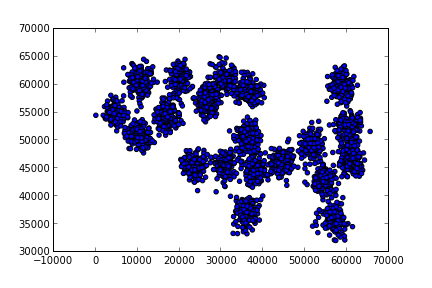
\includegraphics[height=6cm]{kmeans_1.png}
\begin{minted}[fontsize=\footnotesize]{python}
def euc_to_clusters(x,y):
    return np.sqrt(np.sum((x-y)**2, axis=1))

class KMeans():
    def __init__(self,k,iter):
        self.k = k
        self.iter = iter
    def fit(self,X):
        # her veri noktasi icin rasgele kume merkezi ata
        labels = [random.randint(0,self.k-1) for i in range(X.shape[0])]
        self.labels_ = np.array(labels)
        self.centers_ = np.zeros((self.k,X.shape[1]))
        for i in range(self.iter):
            # yeni kume merkezleri uret
            for j in range(self.k):
                # eger kume j icinde hic nokta yoksa, ortalama (mean)
                # hesabi yapma, cunku o zaman nan degeri geliyor, ve
                # hesabin geri kalani bozuluyor.
                if len(X[self.labels_ == j]) == 0: continue
                center = np.mean(X[self.labels_ == j],axis=0)
                self.centers_[j,:] = center
            # her nokta icin kume merkezlerine gore kume atamasi yap
            self.labels_ = []
            for point in X:
                c = np.argmin(euc_to_clusters(self.centers_, point))
                self.labels_.append(int(c))

            self.labels_ = np.array(self.labels_)
\end{minted}

\begin{minted}[fontsize=\footnotesize]{python}
cf = KMeans(k=5,iter=20)
cf.fit(data)
print cf.labels_
\end{minted}

\begin{verbatim}
[2 2 2 ..., 0 0 0]
\end{verbatim}

Ustteki sonucun icinde iki ana vektor var, bu vektorlerden birincisi icinde
2,0, gibi sayilar goruluyor, bu sayilar her noktaya tekabul eden kume
atamalari.  Ikinci vektor icinde iki boyutlu $k$ tane vektor var, bu
vektorler de her kumenin merkez noktasi. Merkez noktalarini ham veri
uzerinde grafiklersek (kirmizi noktalar)

\begin{minted}[fontsize=\footnotesize]{python}
plt.scatter(data[:,0],data[:,1])
plt.hold(True)
plt.ylim([30000,70000])
for x in cf.centers_: plt.plot(x[0],x[1],'rd')
plt.savefig('kmeans_2.png')
\end{minted}

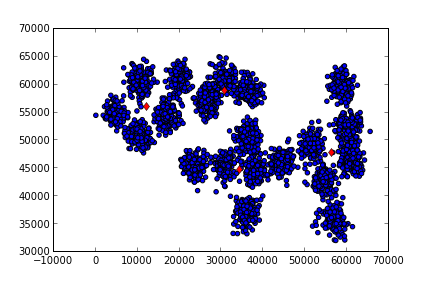
\includegraphics[height=6cm]{kmeans_2.png}

Goruldugu gibi 5 tane kume icin ustteki merkezler bulundu. Fena
degil. Eger 10 dersek

\begin{minted}[fontsize=\footnotesize]{python}
cf = KMeans(k=10,iter=30)
cf.fit(data)
plt.scatter(data[:,0],data[:,1])
plt.ylim([30000,70000])
plt.hold(True)
for x in cf.centers_: plt.plot(x[0],x[1],'rd')
plt.savefig('kmeans_3.png')
\end{minted}

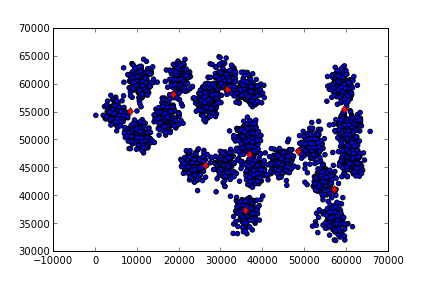
\includegraphics[height=6cm]{kmeans_3.png}

Kategorik ve Numerik Iceren Karisik Veriler

Bazen verimiz hem kategorik hem de numerik degerler iceriyor olabilir,
KMeans yeni kume merkezlerini hesaplarken ortalama operasyonu
kullandigi icin sadece numerik veriler uzerinde calisabilir (kategorik
verilerin nasil ortalamasini alalim ki?). Bu durumda ne yapacagiz?

Bir secenek su olabilir, kategorik her kolonu her degisik degeri bir
yeni kolona tekabul edecek sekilde saga dogru acariz, ve o degerin
yeni kolonuna 1 degeri digerlerine 0 degeri veririz. Bu kodlamaya
1-in-q kodlamasi, 1-in-n kodlamasi, ya da Ingilizce one-hot encoding
ismi veriliyor.

Ornek olarak UCI veri bankasindan Avustralya Kredi Verisine bakalim:

\begin{minted}[fontsize=\footnotesize]{python}
import pandas as pd
df = pd.read_csv("crx.csv")
print df[:2]
\end{minted}

\begin{verbatim}
  A1     A2    A3 A4 A5 A6 A7    A8 A9 A10  A11 A12 A13    A14  A15 A16
0  b  30.83  0.00  u  g  w  v  1.25  t   t    1   f   g  00202    0   +
1  a  58.67  4.46  u  g  q  h  3.04  t   t    6   f   g  00043  560   +
\end{verbatim}

Bu veride A1, A2, gibi kolon isimleri var, kategorik olanlarda 'g','w' gibi
degerler goruluyor. Bu kolonlari degistirmek icin

\begin{minted}[fontsize=\footnotesize]{python}
from sklearn.feature_extraction import DictVectorizer
def one_hot_dataframe(data, cols, replace=False):
    vec = DictVectorizer()
    mkdict = lambda row: dict((col, row[col]) for col in cols)
    vecData = pd.DataFrame(vec.fit_transform(data[cols].apply(mkdict, axis=1)).toarray())
    vecData.columns = vec.get_feature_names()
    vecData.index = data.index
    if replace is True:
        data = data.drop(cols, axis=1)
        data = data.join(vecData)
    return (data, vecData, vec)

df2, _, _ = one_hot_dataframe(df, ['A1','A4','A5','A6','A7','A9','A10','A12','A13'], replace=True)
print df2.ix[0]
\end{minted}

\begin{verbatim}
A2        30.83
A3         0.00
A8         1.25
A11        1.00
A14      202.00
A15        0.00
A16        1.00
A10=f      0.00
A10=t      1.00
A12=f      1.00
A12=t      0.00
A13=g      1.00
A13=p      0.00
A13=s      0.00
A1=a       0.00
A1=b       1.00
A4=l       0.00
A4=u       1.00
A4=y       0.00
A5=g       1.00
A5=gg      0.00
A5=p       0.00
A6=aa      0.00
A6=c       0.00
A6=cc      0.00
A6=d       0.00
A6=e       0.00
A6=ff      0.00
A6=i       0.00
A6=j       0.00
A6=k       0.00
A6=m       0.00
A6=q       0.00
A6=r       0.00
A6=w       1.00
A6=x       0.00
A7=bb      0.00
A7=dd      0.00
A7=ff      0.00
A7=h       0.00
A7=j       0.00
A7=n       0.00
A7=o       0.00
A7=v       1.00
A7=z       0.00
A9=f       0.00
A9=t       1.00
Name: 0, dtype: float64
\end{verbatim}

Islem sonucunda A12=f mesela icin 1 verilmis, ama A12=t (ve diger her
mumkun deger icin yani) 0 degeri verilmis (sadece bu tek satir
icin). Boylece kategorik veriyi sayisal hale cevirmis olduk.

Fakat isimiz bitti mi? Hayir. Simdi KMeans bu tur veriyle acaba duzgun
calisir miydi onu kendimize soralim. Icinde pek cok 0, bazen 1 iceren 
veri satirlari arasinda uzaklik hesabi yapmak ise yarar mi?

Yapay Ogrenim literaturunde bu tur veriler uzerinde kosinus benzerligi
(cosine similarity) kullanmak daha yaygindir. Bu konuyu {\em SVD, Toplu
Tavsiye} yazisinda daha iyi gorebilirsiniz. Kosinus benzerligi bize
0 ile 1 arasinda bir deger dondurur. Benzerligi uzakliga cevirmek icin
basit bir sekilde 1-benzerlik formulunu kullanabiliriz.

O zaman karisik veriler uzerinde KMeans kullanmak icin, verinin en
bastan numerik olan kismi icin Oklit uzakligi, diger kalan kismi icin
kosinus uzakligi kullanabiliriz. Her iki kisimdan elde edilen uzaklik
degerlerini toplariz.

\begin{minted}[fontsize=\footnotesize]{python}
from numpy import linalg as la
import pandas as pd, os
import scipy.sparse as sps
import numpy, random

def cos_dist(inA,inB):
    num = float(np.dot(inA.T,inB))
    denom = la.norm(inA)*la.norm(inB)
    sim = 0.5+0.5*(num/denom)
    return 1. - sim

def mixed_to_clusters(vect,x,euc_n,weights):
    res1 = euc_to_clusters(vect[:,0:euc_n],x[0:euc_n])
    res2 = map(lambda y: cos_dist(x[euc_n:],y), vect[:,euc_n:])
    res = np.array(res1)*weights[0] + np.array(res2)*weights[1]
    return res

class MixedKMeans():
    def __init__(self,k,iter,euc_n,weights=[1.,1.]):
        self.k = k
        self.iter = iter
        self.euc_n = euc_n
        self.weights = weights
    def fit(self,X,iter=10):
        labels = [random.randint(0,self.k-1) for i in range(X.shape[0])]
        self.labels_ = np.array(labels)
        self.centers_ = np.zeros((self.k,X.shape[1]))
        for i in range(self.iter):
            for j in range(self.k):
                if len(X[self.labels_ == j]) == 0: continue
                center = np.mean(X[self.labels_ == j],axis=0)
                self.centers_[j,:] = center
            self.labels_ = []
            for point in X:
                c = np.argmin(mixed_to_clusters(self.centers_, \
                              point, self.euc_n,self.weights))
                self.labels_.append(int(c))

            self.labels_ = np.array(self.labels_)
\end{minted}

\begin{minted}[fontsize=\footnotesize]{python}
df = pd.read_csv("crx.csv",sep=',',na_values=['?'])
df = df.dropna()

df['A16'] = df['A16'].str.replace('+','1')
df['A16'] = df['A16'].str.replace('-','0')
df['A16'] = df['A16'].astype(int)

df2, _, _ = one_hot_dataframe(df, ['A1','A4','A5','A6','A7','A9','A10','A12','A13'], replace=True)
df2 = df2.drop('A16',axis=1)

df2 = np.array(df2)

# veriyi normalize et, ortalama cikar ve standart sapmaya bol
df2 -= np.mean(df2, axis=0)
df2 /= np.std(df2, axis=0)

cf = MixedKMeans(2,iter=10,euc_n=6,weights=[1.,3.])
cf.fit(df2)

labels_true = np.array(df['A16'])
labels_pred = cf.labels_
match = np.sum((labels_true == labels_pred).astype(int))
print float(match)/len(df)
\end{minted}

\begin{verbatim}
0.816232771822
\end{verbatim}

Bu veri icinde iki tane kume vardi, kumeler A16 kolonunda + ya da - olarak
isaretli. Kumeleme takip edilmeyen (unsupervised) bir Yapay Ogrenim
metotududur, hangi noktanin hangi kumeye ait oldugunu onceden bilmeyiz,
ornek veri setini kullanirken bu isaretleri gormemezlikten geliyoruz,
sadece kontrol amacli olarak sonradan bu isaretlere bakiyoruz. Ve ustteki
kod ile yuzde 82 civari (bazen 82, bazen 18 degeri gelebilir, cunku kume
atamalari ``1. kume'' ya da ``0. kume'' arasinda bir secim yapamaz, sadece
onlarin ayri kume olduklarini bulabilir, tahminler bu sebeple bazen tam
tersi cikabiliyor, fakat bu cok onemli degil) oraninda bir basariyla dogru
kumeyi bulabilmisiz.

Parametre olarak gecilen \verb!euc_n! degiskeni her veri noktasi icin "ilk kac
noktanin numerik" oldugunu belirtiyor. Boylece uzaklik fonksiyonu sadece
o kisimda Oklit uzakligi kullaniyor. Peki numerik degerler niye hep basta?
Sebep \verb!one_hot_dataframe! cagrisinin yeni kolonlari yaratirken eskileri
silmesi ve eklenen yeni kolonlarin hep en sona konmasi, boylece en bastakiler
hep numerik kolon olacak!

Agirliklar

Oklit ve kosinus uzakliklarini birbirine toplarken, birine digerinden
daha fazla agirlik vermek mumkun, belki de bir veri seti icin numerik
veriler kategorik olanlardan daha onemli olabilir, bu durumda
agirliklari, mesela ustte 1'e 3 olarak tanimladik, Oklit uzakligina 3
kat daha fazla onem / agirlik vermis oluruz cunku kategorik verileri 3
kat daha "fazlalastiriyoruz", "uzaklastiriyoruz". Tabi bu konuyu
degisik bir acidan gormek te mumkun, eger kategorik kismin sayilari
numerik olanlar ile ayni olcekte degilse, carparak her iki kismi
esitlemis oldugumuz da soylenebilir. Her neyse - agirliklarin ne
oldugu tahmin, deneme / yanilma ile bulunabilir, her veri setine gore
degisik olacaklardir.

Normalize Etmek

Ustteki ornekte veriyi 1-in-n kodlamasiyla cevirdikten sonra bir de
normalize ettik, yani her kolon bazinda o kolonun ortalamasini o
kolondaki tum degerlerden cikarttik ve standart sapmaya bolduk,
boylece her kolonu 0 etrafinda ortalayip onun iki tarafina dusebilecek
-/+ degerleri kucultuyoruz. Bu veriyi bir tur "sekle sokma" islemidir,
ne zaman kullanilacagi tecrubeyle ortaya cikar, mesela ustteki karisik
veride bunun isleyebilecegini tahmin ettik. 

Kume sayisini bulmak

KMeans'e kume sayisinin onceden verilmis olmasi gerekiyor, ve bu
sayiyi KMeans baglaminda bastan bilmiyoruz. Bu sayiyi bir sekilde
bulmanin yolu olamaz mi?

Boyut azaltma teknigi SVD yardimci olabilir. SVD sonrasi gelen
matrisin "onemli" kolonlarinda daha azaltilmis bir veri seti elde
edebiliriz, bu veride en basta olan kolonlar en onemli olanlardir, ve
bu kolonlari, mesela ilk ikisini alarak ekrana basabiliriz. Avustralya
Kredi setinde bunu yaparsak sunu goruruz:

\begin{minted}[fontsize=\footnotesize]{python}
import scipy.linalg as lin
u,s,vt=lin.svd(df2) # normalize edilmis veri uzerinde
plt.plot(u[:,0], u[:,1],'.')
plt.savefig('kmeans_4.png')
\end{minted}

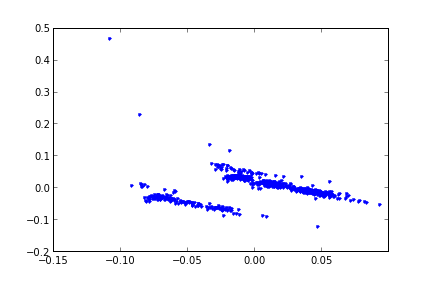
\includegraphics[height=6cm]{kmeans_4.png}

Iki tane ana blok oldugu acik bir sekilde goruluyor. Demek ki kume sayisi
k = 2 kullanmak gerekir. 

Bazi ek notlar

[1] \url{http://en.wikipedia.org/wiki/Determining_the_number_of_clusters_in_a_data_set}

[2] \url{nbviewer.ipython.org/url/cbcb.umd.edu/~hcorrada/PML/src/kmeans.ipynb}


\end{document}
